\documentclass[a4paper]{article}

\usepackage{geometry}
\usepackage{amsmath}
\usepackage{fontspec}
\usepackage{graphicx}
\usepackage{minted}

\usepackage{polyglossia}
\setmainlanguage[variant=american]{english}

\usepackage{hyperref}
\usepackage{subcaption}

\DeclareMathOperator*{\argmin}{arg\,min}
\DeclareMathOperator*{\argmax}{arg\,max}

\title{INF4300 -- Mandatory project -- Part 2}
\author{Bjørn Rustad}
\date{\today}

\begin{document}

\maketitle

\section{Choosing GLCM parameters}

\begin{figure}[h]
    \centering
    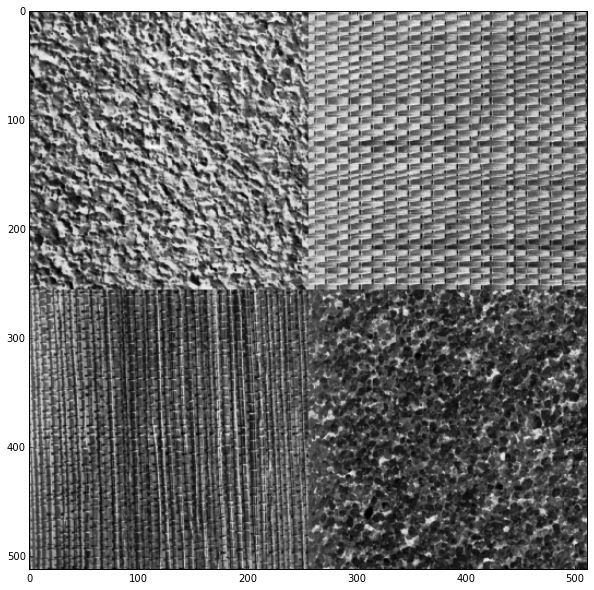
\includegraphics[width=0.25\textwidth]{mosaic1.png}
    \caption{The training image containing four different textures.}
    \label{fig:train_tex}
\end{figure}

The images we are analysing are similar to the mosaics in part 1 of the
project. The training image can be seen in Figure~\ref{fig:train_tex},
where the top right and bottom left texture are very regular and
directional, while the other two are more grainy and randomly directed.

GLCM matrices are given for the four different textures, for four sets
of parameters $(dx, dy) = \{(0, -1), (1, 0), (-1, -1), (1, -1)\}$. The
number of levels is always $G = 16$. This is what we have to work with,
but in my opinion it seems strange to only have step sizes in $\{-1, 0,
1\}$ when some of the textures have obvious structures of larger sizes
(like the upper right and lower left).

\begin{figure}
    \centering
    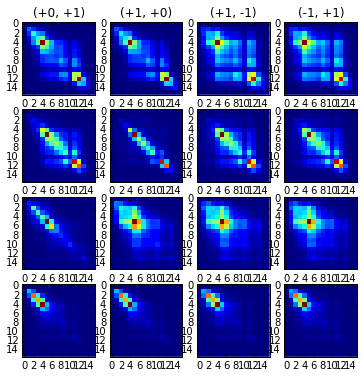
\includegraphics[width=0.5\textwidth]{glcm_mat.png}
    \caption{%
        GLCM matrices visualized for the different parameters. The rows
        correspond to the different textures, and the GLCM parameters
        for each column are shown on the top.
    }
    \label{fig:glcm_mat}
\end{figure}

Figure~\ref{fig:glcm_mat} shows the different GLCM matrices visualized
for the different textures. Each row corresponds to one texture. First
we observe that there is a lot of similarities between the feature
matrices, so we can't go \emph{too} wrong when we choose two to continue
working with. I choose feature 2 $(+1, +0)$, because it seems to best
separate texture 2 from the other textures. Next I choose feature 1
because it differs the most from the other features, and we want
features that give as much information as possible. The downside of
feature 1 is that texture 3 and 4 look similar, but hopefully feature 2
can make up for that.

Thus I choose to work with feature 1 and 2, i.e.\ $(dx, dy) = \{(1, 0),
(0, 1)\}$.

\section{GLCM quadrant features}

We here look at features calculated as the fraction of weight
concentrated in four different quadrants $Q_1, Q_2, Q_3, Q_4$ of the
GLCM matrices. The GLCM matrices are of dimension 16-by-16 and thus
\begin{equation}
    Q_1 = \frac{\sum_{i=1}^8 \sum_{j=1}^8 P(i, j)}{\sum_{i=1}^{16}
    \sum_{j=1}^{16} P(i, j)}
\end{equation}
and similarly for the other quadrants. Note that our GLCM matrices are
symmetric and thus $Q_2 = Q_3$, and we only consider one of them from
here on.

Looking at the GLCM matrices (column 2 and 3) in
Figure~\ref{fig:glcm_mat}, it seems like these features can do an OK job
at separating the different textures. The fourth quadrant $Q_4$ seems
like it can separate the first two from the last two textures. Possible
problems might be that texture 1 is similar to texture 2, and that
texture 3 is similar to texture 4.

A lot of weight is contained inside the first quadrant $Q_1$, and thus
I choose to subdivide this quadrant with hopes that the extra features
will help differentiating between textures 1 and 2, and also between
textures 3 and 4. I denote the subdivision $Q_1 = Q_{11} \cap Q_{12}
\cap Q_{13} \cap Q_{14}$, and also here because of symmetry $Q_{12} =
Q_{13}$. Since $Q_{1}$ can be fully described by the features of from
the subdivision, we do not need it anymore. For each set of GLCM
parameters we then have the features $[Q_{11}, Q_{12}, Q_{14}, Q_{2},
Q_{4}]$.

\section{Selecting and implementing a subset of features}

\begin{figure}
    \centering
    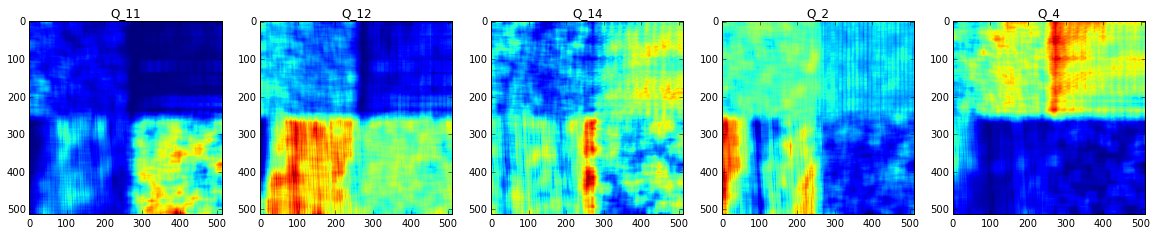
\includegraphics[width=\textwidth]{g1feats.png}
    \caption{%
        Selected quadrant features for the GLCM with parameters $(dx,
        dy) = (1, 0)$ and $G=16$.
    }
    \label{fig:g1feats}
\end{figure}

\begin{figure}
    \centering
    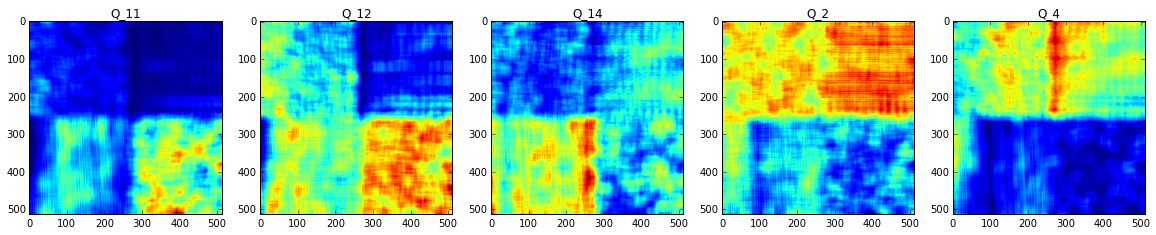
\includegraphics[width=\textwidth]{g2feats.png}
    \caption{%
        Selected quadrant features for the GLCM with parameters $(dx,
        dy) = (0, 1)$ and $G=16$.
    }
    \label{fig:g2feats}
\end{figure}

Figure~\ref{fig:g1feats} and \ref{fig:g2feats} show the five currently
selected quadrant features for the two sets of GLCM parameters. Within
each GLCM parameter, I would say the features show sufficient variation.
However, there are a lot of similarities from Figure~\ref{fig:g1feats}
to Figure~\ref{fig:g2feats}, i.e.\ between the GLCM parameter sets.
Looking closer though, we can see some variation, and it is really
$Q_{11}$ and $Q_4$ that show the least variation.

\begin{figure}
    \centering
    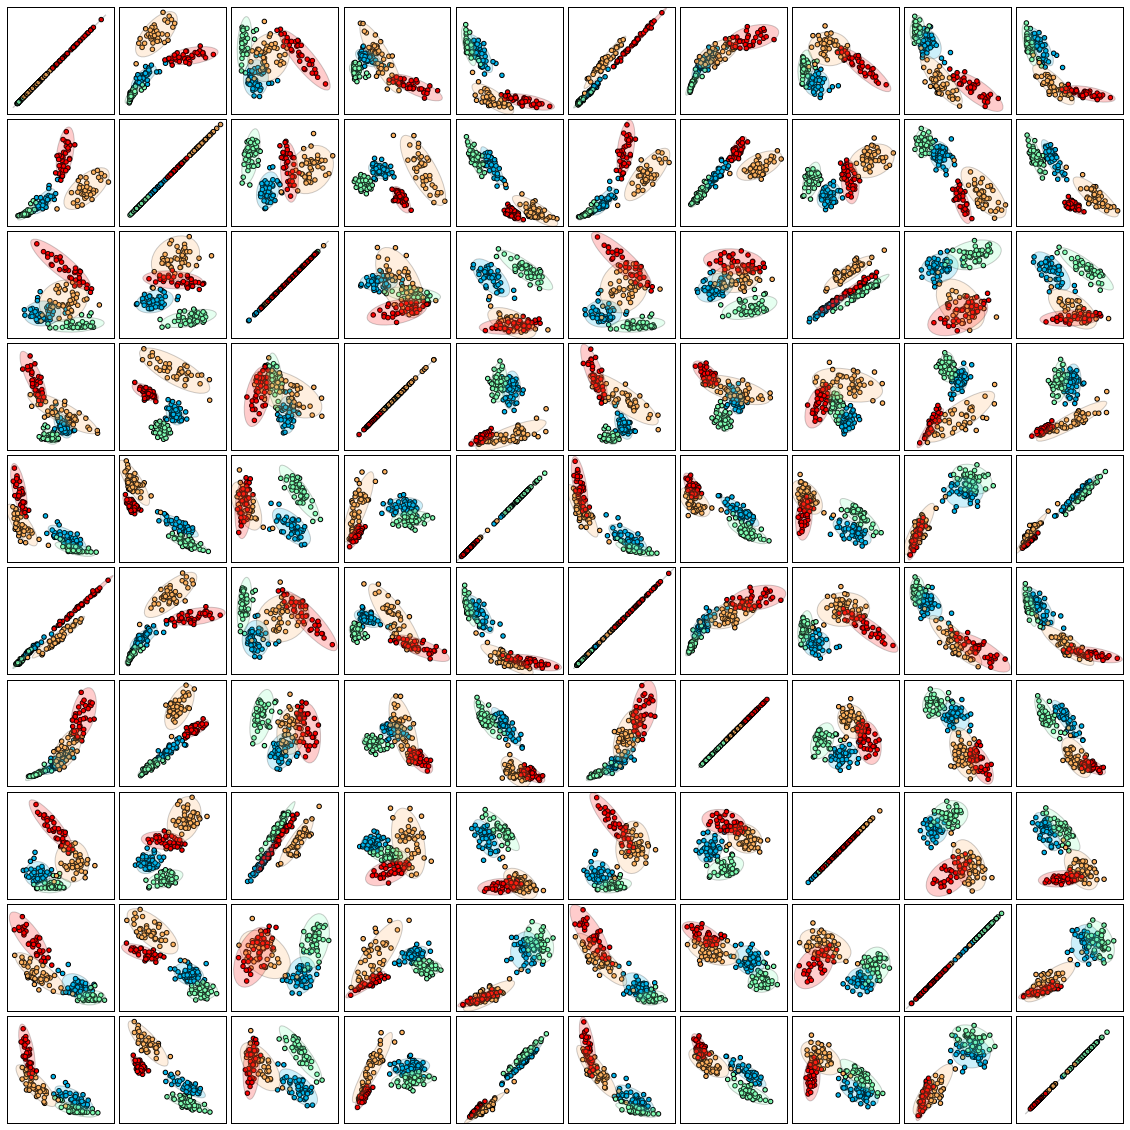
\includegraphics[width=\textwidth]{feat_comp.png}
    \caption{%
        A scatter plot for each combination of two features. As the
        training set contains 166253 pixels, we only plot a small,
        random selection of them.
    }
    \label{fig:feat_comp}
\end{figure}

In lack of a better notation I denote our ten features by $Q_{k}^{(dx,
dy)}$ and order them as
\begin{equation}
    [Q^{(1,0)}_{11}, Q^{(1,0)}_{12}, Q^{(1,0)}_{14}, Q^{(1,0)}_{2},
        Q^{(1,0)}_{4}, Q^{(0,1)}_{11}, Q^{(0,1)}_{12}, Q^{(0,1)}_{14},
    Q^{(0,1)}_{2}, Q^{(0,1)}_{4}]
\end{equation}

Figure~\ref{fig:feat_comp} we can see a scatter plot of each pairwise
combination of the ten features. Only a random small selection of the
training pixels in each class are shown. We can see that the first
feature $Q^{(1,0)}_{11}$ is very similar to the sixth feature
$Q^{(0,1)}_{11}$ from the linearity of their scatter plot. The features
$Q^{(1,0)}_{4}$ and $Q^{(0,1)}_{4}$ are also very similar. We could
probably safely drop one from each of these two pairs.

\section{Implementing a Gaussian classifier}

I implement a Gaussian classifier as described in the lecture notes. The
idea is that the feature vectors of pixels in a class belong to some
multivariate Gaussian distribution, with its own mean, and possibly with
its own covariance matrix. These parameters of the Gaussian
distributions of the different classes need to be estimated from our
training data. If feature vector $i$ in with class $c$ is denoted by
$x^{(c)}_i$ we estimate the mean of the class as
\begin{equation}
    \hat{\mu}_c = \frac{1}{N_c} \sum_i x^{(c)}_i.
\end{equation}

For estimating the covariance matrix we have several options, depending
on what we assume about our data, and also by how much training data we
have available. The easiest is to estimate one single diagonal
covariance matrix for all the training data. A model a little more
complex is obtained by instead estimating a full covariance matrix for
all the traning data. The most complex model is obtained by etimating a
full covariance matrix for each class. Of course other combinations are
also possible.

Complex models are more flexible, but also have more parameters to
estimate, requiring more training data, and having a larger risk of
overfitting to the training data. A full covariance matrix is symmetric
and thus has $p \times (p+1) / 2$ free parameters, where $p$ is the
number of features, in our case 10. Thus we have 55 parameters per
covariance matrix. Each class also has a mean, needing $p = 10$
parameters. Thus each of the four classes has 65 parameters, and we have
260 parameters in total. As we have 166253 training pixels, this goes
well within the rule of thumb of 10 samples per feature per class.

Thus I choose to implement one full covariance matrix for each class.
This can be estimated for class $c$ by summing over all the training
samples in the class
\begin{equation}
    \hat{\Sigma}_c = \frac{1}{N_c} \sum_i (x^{(c)}_i -
    \hat{\mu}_c)(x^{(c)}_i - \hat{\mu}_c)^T.
\end{equation}

To predict the class of a test sample we calculate the probability of it
belonging to each of the four classes, and classify it as belonging to
the most probable class. The posterior probability of the class $\omega$
of the feature vector $x$ is
\begin{equation}
    p(\omega = c \mid x) = \frac{p(x \mid \omega = c) \cdot p(\omega =
    c)}{p(x)}
\end{equation}

We are only interested in the relative probability of the classes, so we
can disregard $p(x)$ as it is constant for a given $x$. The prior
probability of each class $p(\omega = c)$ is estimated by the fraction
of training samples from that class
\begin{equation}
    p(\omega = c) = \frac{N_c}{\sum_i N_i}
\end{equation}

The likelihood of observing the feature vector $x$ given the class $c$
is given by the Gaussian multivariate distribution
\begin{equation}
    p(x \mid \omega = c) = \frac{1}{(2\pi)^{n/2}
    \left|{\hat{\Sigma}_c}\right|^{1/2}} \exp\left({-\frac{1}{2} (x -
    \hat{\mu}_c)^T\hat{\Sigma}_c^{-1}(x - \hat{\mu}_c)}\right).
\end{equation}

Some tricks are made in the calculation of these probabilities. Since
the logarithm is a monotonically increasing function we can use that
\begin{equation}
    \hat{c} = \argmax_c p(\omega = c \mid x) = \argmax_c \log p(\omega =
    c \mid x)
\end{equation}
which in turn simplifies to
\begin{equation}
    \hat{c} = \argmax_c \left( -\frac{1}{2} \log |\hat{\Sigma}_c| -\frac{1}{2}
    (x - \hat{\mu}_c)^T\hat{\Sigma}_c^{-1}(x - \hat{\mu}_c) + \log
    p(\omega = c)\right).
\end{equation}
To speed up computations, terms not containing the feature vector $x$
can be extracted and precalculated once for each class $c$.

\section{Training the classifier}

I train the implemented classifier on the training set, with the classes
as described in the \texttt{training\_mask} file, and the 10 different
features as selected previously. Note that I pad the training and
testing images by reflecting the image around the border such that I
obtain GLCM feature images of the same size as the original images.

I obtain a training accuracy of 100\% meaning that the confusion matrix
is the identity matrix, and not very interesting to inspect. The
question is now whether we have overfitted to the training set.

\section{Testing the classifier}

\begin{figure}
    \centering
    \begin{subfigure}[b]{0.23\textwidth}
        \centering
        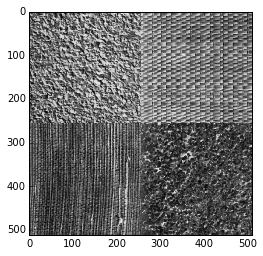
\includegraphics[width=\textwidth]{mosaic2_test.png}
        \caption{%
            Test image.
        }
    \end{subfigure}
    ~
    \begin{subfigure}[b]{0.23\textwidth}
        \centering
        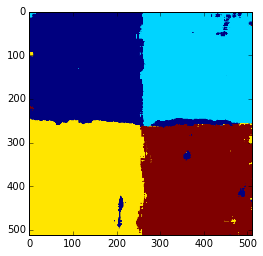
\includegraphics[width=\textwidth]{mosaic2_pred.png}
        \caption{%
            Predicted classes.
        }
    \end{subfigure}
    \caption{%
        Test mosaic 2 and the predicted classes.
    }
    \label{fig:test2}
\end{figure}

\begin{figure}
    \centering
    \begin{subfigure}[b]{0.23\textwidth}
        \centering
        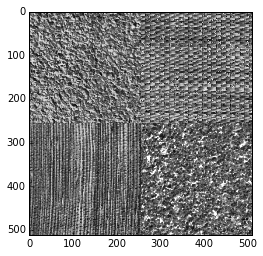
\includegraphics[width=\textwidth]{mosaic3_test.png}
        \caption{%
            Test image.
        }
    \end{subfigure}
    ~
    \begin{subfigure}[b]{0.23\textwidth}
        \centering
        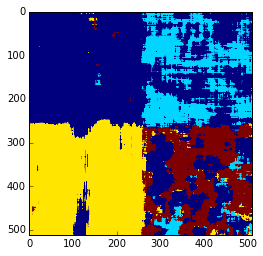
\includegraphics[width=\textwidth]{mosaic3_pred.png}
        \caption{%
            Predicted classes.
        }
    \end{subfigure}
    \caption{%
        Test mosaic 3 and the predicted classes.
    }
    \label{fig:test3}
\end{figure}

I test the classifier on the two testing images provided. The results
are visualized in Figures~\ref{fig:test2} and \ref{fig:test3} with one
color representing each class. It is clear that the classifier performs
pretty well on test image 2, while not so great on test image 3.

\begin{table}
    \caption{Confusion matrix of test mosaic 2 with true labels vs.\
    predicted labels.}
    \centering
    \begin{tabular}{l | r | r | r | r | r}
        \small{True \textbackslash\ Pred.} & 1 & 2 & 3 & 4 & Sum \\ \hline
        1 & 64268 &    346 &    863 &     59 &   65536 \\ \hline
        2 & 3222  & 62301  &     3  &    10  &  65536  \\ \hline
        3 & 694   &    0   & 64410  &   432  &  65536  \\ \hline
        4 & 1587  &   146  &  1540  & 62263  &  65536  \\ \hline
        Sum & 69771 &  62793 &  66816 &  62764 &  262144
    \end{tabular}
    \label{tab:conf2}
\end{table}

\begin{table}
    \caption{Confusion matrix of test mosaic 3 with true labels vs.\
    predicted labels.}
    \centering
    \begin{tabular}{l | r | r | r | r | r}
        \small{True \textbackslash\ Pred.} & 1 & 2 & 3 & 4 & Sum \\ \hline
        1 &    64669 &   160 &   430 &   277 &  65536 \\ \hline
        2 &    \emph{33505} & 31996 &     0 &    35 &  65536 \\ \hline
        3 &     4522 &     0 & 60881 &   133 &  65536 \\ \hline
        4 &    \emph{24983} &  4513 &  3117 & 32923 &  65536 \\ \hline
        Sum & \emph{127679} & 36669 & 64428 & 33368 & 262144
    \end{tabular}
    \label{tab:conf3}
\end{table}

Table \ref{tab:conf2} shows the confusion matrix of test mosaic 2
(Figure~\ref{fig:test2}). We see that the overall performance is good.
We have the highest confusion for true class 2 pixels that are predicted
to be of class 1.

Table~\ref{tab:conf3} shows the confusion matrix of test mosaic 3
(Figure~\ref{fig:test3}). There is more confusion here. Over half of the
true class 2 pixels and a lot of the true class 4 pixels are confused
to be of class 1, resulting in that class 1 contains twice as many
pixels as it should.

Looking at the mosaics, it appears that the shadings of the two bottom
textures are very different in the two test images. If we are only
interested in classifying textures, shadings should not matter of
course. This could possibly be improved by applying some kind of
histogram normalization to the training and testing images. Another
option is to augment the training set by varying the brightness of the
training image, yielding a larger training set with more shading
variations.

Upon closer inspection it seems that the top right texture of test
mosaic 3 has quite a bit of salt and pepper noise. A simple median
filter works well at removing this kind of noise, and should for
concistency probably be applied to all the images, both training and
testing.

\begin{figure}
    \centering
    \begin{subfigure}[t]{0.23\textwidth}
        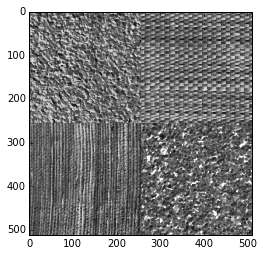
\includegraphics[width=\textwidth]{median_filt.png}
        \caption{%
            Median filtered test image 3.
        }
    \end{subfigure}
    ~
    \begin{subfigure}[t]{0.23\textwidth}
        \centering
        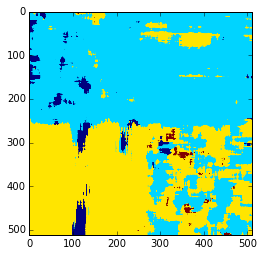
\includegraphics[width=\textwidth]{median_filt_pred.png}
        \caption{%
            Predicted classes.
        }
    \end{subfigure}
    \caption{%
        Predictions on a median filtered test image 3 using a 3-by-3
        median filter.
    }
    \label{fig:median_filt_pred}
\end{figure}

Figure~\ref{fig:median_filt_pred} shows the results of running our
classifier on the test image 3 when it has been filtered using a 3-by-3
median filter. Overall, the results are worse, although more of the
second texture (which initially contained noise) is classified
correctly.

Many improvements are possible, but my hypothesis is that more
adaptation of the GLCM $dx$ and $dy$ parameters, as well as some initial
pre-processing and normalization of the training and testing images
would be a good place to start. Or possibly using completely different
features.

\appendix

\section{Code}
\label{app:code}

\subsection{GLCM calculation}

Functions for calculating the GLCM matrices of a single patch, or for a
whole image, as well as some different GLCM features.

\inputminted[fontsize=\footnotesize]{python}{../glcm.py}

\subsection{Gaussian classification}

A simple Gaussian classifier supporting different ways of calculating
the covariance matrices.

\inputminted[fontsize=\footnotesize]{python}{../gaussian.py}

\subsection{Experimentation}

Feature extraction, inspection, and classification listed in the order
described in the text.

\inputminted[fontsize=\footnotesize]{python}{test.py}

\end{document}

